% Preview source code

%% LyX 2.3.5.2 created this file.  For more info, see http://www.lyx.org/.
%% Do not edit unless you really know what you are doing.
\documentclass[english]{article}
\usepackage[T1]{fontenc}
\usepackage[latin9]{inputenc}
\usepackage{amsmath}
\usepackage{graphicx}
\usepackage{babel}
\begin{document}
\noindent \tableofcontents{}

\noindent \newpage{}

\part{\emph{Agile Software Development}}

\section{\emph{Agile Outline}}
\begin{enumerate}
\item Customer Satisfaction by early and continuous delivery of valuable
software.
\item Welcome changing requirements, even in late development.
\item Deliver working software frequently.
\item Close, daily cooperation between business people and developers.
\item Projects are built around motivated individuals who should be trusted.
\item Face to face conversation is the best form of communication.
\item Working software is the primary measure of progress.
\item Sustainable development, able to maintain a constant pace.
\item Continuous attention to technical excellence and good design.
\item Simplicity - the art of maximising the amount of work not done is
essential
\item Best architectures and designsemerge from self organising teams.
\item The team regularly reflects on how to become more effective and adjusts
accordingly.
\end{enumerate}
%

\subsection{\emph{How can one enforce Agile Software Development?}}
\begin{itemize}
\item Break product development into small increments that minimise the
amount of up front planning and designs.
\item Enforce iterations or sprints, which involves a multi-disciplinary
team working on: planning, analysis, design, coding, unit testing,
and acceptance testing.
\item Fail often and fail early with incremental development; working software
is the primary measure of progress.
\item Enforce Face to face communication with team members and stakeholders.
\begin{itemize}
\item Delegate a customer representative to act on behalf of the opinions
of stakeholders.
\item Customer opinions determine the direction of the next sprint / workflow.
\end{itemize}
\item Daily standup: 15 minute session where members collectively review
how they are progressing towards their goal, and note criticisms and
improvements. 
\item Focus on quality of architecture:
\begin{itemize}
\item Continuous integration.
\item Unit testing, test driven development.
\item Pair programming.
\item Enforcing design patterns onto the architecture.
\end{itemize}
\end{itemize}

\subsection{\emph{Where is ASD appropriate?}}
\begin{itemize}
\item Complex systems with dynamic, non deterministic and non linear characteristics,
since accurate estimates and stable plans are hard to get in early
stages. 
\item In a desire to reduce the \emph{leap of faith }that is needed before
any evidence of value can be obtained, in system development.
\end{itemize}
\noindent 
%
\noindent \newpage{}

\part{\emph{Legal, Ethical and Professional Conduct}}

\noindent There are a number of \emph{standards }which highlight a
set of axioms by which software engineers should operate, to encourage
ethical and legal behaviour:

\section{\emph{ACM (Association for Computing Machinery) {[}58,68{]}}}

ACM are the worlds largest computing society which provide activities,
guidance and principles to support professional growth.

\subsection{\emph{General Ethical Principles:}}
\begin{itemize}
\item Contribute to society and to human well being, acknowleding that all
people are stakeholders in computing.
\begin{itemize}
\item Avoid harm.
\item Be honest and trustworthy.
\item Be fair and take action not to discriminate.
\item Respect the work required to produce new ideas, inventions, creative
works, and computing artifacts.
\item Respect privacy.
\item Honor confidentiality.
\end{itemize}
\end{itemize}

\section{\emph{IEEE (Institute of Electrical and Electronics Engineers) {[}69,74{]}}}

\noindent IEEE is the worlds largest techincal professional organisation
which enforces 8 practices which software engineers should take with
regards to ethics and professional practices.

\subsection{\emph{IEE Code of Ethics.}}
\begin{itemize}
\item Upload the highest standards of integrity, responsible behaviour and
ethical conduct in professional activities.
\item Treat all persons fairly and with respect, to not engage in harassment
or discrimination, and to avoid injuring others.
\item Strive to ensure code is upheld by colleagues and co-workers.
\end{itemize}

\section{\emph{BCS {[}75,77{]}}}

\noindent \textbf{\emph{BCS}}\textbf{ }is a Chartered Institute for
IT, and is known as an independant professional body. BCS enforces
four key principles:

\subsection{\emph{General Ethical Principles:}}
\begin{itemize}
\item You make IT/ software for everyone.
\begin{itemize}
\item Address wider societal issues, and upholding standards by conducting
yourself professionally and fairly at all times, to make software
accessible.
\end{itemize}
\item Show what you know, learn what you don't.
\begin{itemize}
\item Keep on learning, continuously learn and develop yourself. You must
know the boundaries of what you do or don't know.
\end{itemize}
\item Respect the organisation or individual you work for.
\begin{itemize}
\item Work with due care and diligence while taking personal and collective
responsibility for your actions; musn't work with conflicts of interest.
\end{itemize}
\item Keep IT real. Keep IT professional. Pass IT on.
\begin{itemize}
\item Uphold the reputation of the profession and encourage others to grow.
\end{itemize}
\end{itemize}

\section{\emph{Research Ethics {[}158,159{]}}}

\subsection{\emph{EIRA {[}https://moodle.bath.ac.uk/pluginfile.php/1469988/mod\_resource/content/6/EIRA1\%20information\%20CC.pdf{]}}}

\noindent Engaging with research involves ethical, legal and professional
considerations.
\begin{itemize}
\item The University of Bath requires the EIRA1 electronic form to be completed
and submitted for review for all projects that involve human participants.
\end{itemize}

\subsection{\emph{Scientific Integrity}}
\begin{itemize}
\item We are expected to act with \textbf{Scientific Integrity}, which enforces
the following principles:
\begin{itemize}
\item \emph{Honesty}\textbf{: }The work you present must be clear and your
intentions must be accurate. Interpretations of data should be clear,
and justifications of data; acknowleding sources, and honesty in the
farming of data.
\item \emph{Rigour}\textbf{: }Research to be rigorous and explore and exhaust
all nodes.
\item \emph{Transparency and open communication}\textbf{: }highlight limitations
of studies and negative results. Must be transparent in your methodologies,
and share criticisms as part of the research process.
\item \emph{Care and respect}: to all beneficiaries of the experiment, including
animals, environments and cultural objects.
\item \emph{Accountability}\textbf{: }Individuals are held to account when
their behaviour falls short of the standards we set.
\end{itemize}
\end{itemize}

\subsection{\emph{Misconduct types:}}
\begin{itemize}
\item \emph{Falsification:}\textbf{ }Manipulating research, equipments or
process; changing data to fit narratives or other goal without any
justification. Remember, negative and null results are valid; it is
a skill to show negative results in a positive light so as to learn
from them.
\item \emph{Plaigarism:}\textbf{ }Using other peoples work and ideas without
giving proper credit to the original source. Violates the rights of
the authors to their intellectual output. 
\item \emph{Fabrication:}\textbf{ }Making up results and recording them
as though they were real. 
\end{itemize}
%

\subsection{\emph{Key Principles of Human Research}}

\subsubsection{\emph{Ethical Principles in Human Research}}

In collecting data from people, there are some basic ethical principles
to consider:
\begin{itemize}
\item \emph{Respect for persons: }Individuals should be treated as autonomous
agents (they can make their own decisions and choices), persons with
diminished responsibilities are entitled to protection.
\item \emph{Beneficence}: The obligation to do no harm, and to maximise
the benefits and reduce the risk.
\item \emph{Justic}e: Do no not deny benefits or impose burdens of research
to people without good reaosn.
\end{itemize}

\subsubsection{\emph{Informed consent}}

The participants should choose what does and does not happen to them.
There are three core elements to informed consent.
\begin{itemize}
\item \emph{Information}: Participants should have access to the risks or
benefits of the research; the ability to ask questions and withdraw
at any time.
\item \emph{Comprehension: }Information must be provided in a coherent manner
which would not curtail the participants ability to make an informed
decision. It is your responsibility to ensure that they have comprehended
the information.
\item \emph{Agreement to Participate: }Valid if given voluntarily and not
through coercion or threat, or undue influence such as an improper
reward (eg a bribe).
\end{itemize}

\subsubsection{\emph{Withdrawal}}
\begin{itemize}
\item Participants must have the right to withdraw:
\begin{itemize}
\item After having read the information sheet.
\item Part way through the study
\item After the study; 
\end{itemize}
\item When working with anonymised data, it may not be possible to extract
an individuals data. Participants must be made aware of this, and
depending on how the data is anonymised, you may want to consider
a \emph{grace period }where you can give participants to withdraw
their data, after which the data will be anonymised.
\end{itemize}

\subsubsection{\emph{Data}}
\begin{itemize}
\item Only collect data that is absolutely necessary.
\item Clearly tell participants what you are recording and why. You must
provide consent if you use images in publications and reports.
\item Anonymise the data if possible (pixelating images).
\item Secure storage of data
\begin{itemize}
\item All participant data should be stored securely on the University drives,
access files with files.bath.ac.uk remotely.
\item All paper data like consent forms should be stored in locked filing
cabinets with clear labels.
\end{itemize}
\end{itemize}

\subsubsection{\emph{Recruitment of Participants}}
\begin{itemize}
\item Use emails, social media, posters, word of mouth.
\item You musn't coerce or pressurise people into taking part. Compensation
should be to compensate their time, not entice them.
\item Must provide fundamental information of the study such as:
\begin{itemize}
\item Study title
\item What will be involved, and duration of study.
\item Criteria for inclusion (eg, healthy adults 18+)
\item Compensation for their time information.
\item Contact information.
\end{itemize}
\end{itemize}

\subsubsection{\emph{Participant Impairments}}

You must consider the impairments of your participants of the study
as the ethical process will take longer and will be more complicated.
Consent could be more problematic if under 18 / those with diminished
responsiblity. 

\subsubsection{\emph{Debriefing}}
\begin{itemize}
\item Thank the participant for their time
\item Provide participants with a full explanation of what was being tested.
\item What were the hypotheses and what were they based upon.
\item Explain how the results will be used.
\item Where they can find more information.
\item Reminder of their right to withdraw.
\end{itemize}
%

\part{\emph{UML Models}}

\section{\emph{UML Case Diagrams}}
\begin{itemize}
\item All application events are inside a box. All external interactions
which produce these events are outside of the box.
\item \textbf{Actors }produce events, in which case a line is drawn from
the actor to the event(s).
\item \textbf{Events }are drawn in circles.
\item \textbf{Event chains }are defined by:
\begin{itemize}
\item <\textcompwordmark <include>\textcompwordmark >, which $\implies$
the next event.
\item <\textcompwordmark <extend>\textcompwordmark >, which could be $\implies$
the next event.
\end{itemize}
\item Events can be defined further by establishing a hierarchy which explains
the proper subtypes of said event.
\item \includegraphics[scale=0.5]{\string"UML Model\string".png}
\end{itemize}

\section{\emph{UML Sequence Diagrams}}

\noindent UML Sequence Diagrams are a type of UQL diagram show how
classes in code interact with each other, in order, namely the sequence
of events. Used to document processes and understand the requirements
of a new program.
\begin{itemize}
\item \textbf{Actors }interact with \textbf{Objects}\textbf{\emph{. }}Objects
are placed in sequential order, and are in squares.
\item \textbf{Lifelines }are vertical dashed lines which show the existence
of the object over time (time axis is vertical).
\item \textbf{Messages }show the messages being sent between objects. These
are indicated with solid lines.
\begin{itemize}
\item \textbf{Return Messages }are dashed lines and are responses to messages.
\end{itemize}
\item \textbf{Alternative Frames} are basically conditional branches, which
symbolises a choice between two message sequences. It is encapsulated
in a box around the target message sequences.
\begin{itemize}
\item 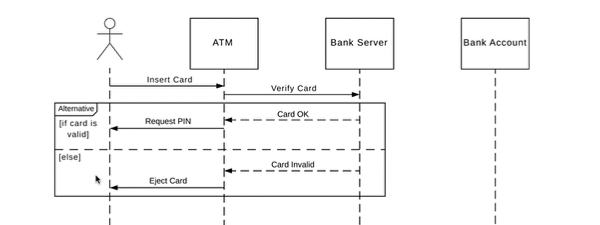
\includegraphics[scale=0.5]{UML_SEQUENCE_1} 
\end{itemize}
\item \textbf{Activation boxes }show when and how long objects perform processes
and go along the lifelines.
\item 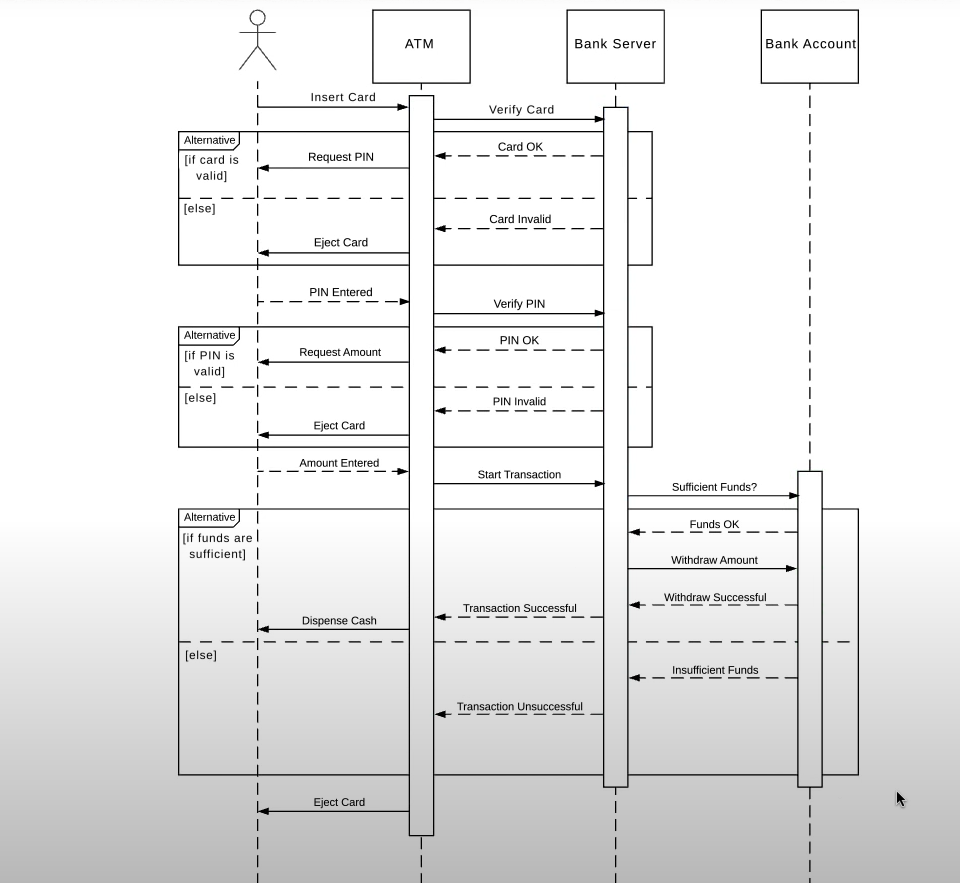
\includegraphics[scale=0.5]{UML_SEQUENCE_2}
\end{itemize}

\section{\emph{Additional Resources}}
\begin{itemize}
\item https://www.uml-diagrams.org/uml-25-diagrams.html
\end{itemize}
\noindent 
%
\noindent \newpage{}

\part{\emph{Data Analysis and Statistics}}

\noindent \newpage{}

\part{\emph{Idea Development}}

\noindent \newpage{}

\part{\emph{Stakeholder Engagement}}

\noindent \newpage
\end{document}

